\section{Regularization Sensitivity}

Figure \ref{fig:epsilon-sweep} plots solver execution times as the regularization parameter \(\varepsilon\) is reduced from \(10^{-2}\) to \(10^{-10}\). Decreasing \(\varepsilon\) drives the \(p\)-Laplacian closer to its singular limit, sharply increasing the stiffness of the nonlinear problem. The grid resolution is fixed at \(N_x = 1000\) with a solver tolerance of \(10^{-6}\). The other parameters are fixed at \(T=0.05\), \(p = 2.5\).

LSODA handles this escalating difficulty effortlessly. Its execution time barely shifts, creeping from 0.078 seconds at \(\varepsilon = 10^{-2}\) to just 0.126 seconds at \(\varepsilon = 10^{-10}\). BDF and Radau are far more sensitive to the tightening physics. Their execution times more than double as \(\varepsilon\) drops, accompanied by heavy increases in internal function and Jacobian evaluations. 

Interestingly, all three solvers hit a hard computational plateau beyond \(\varepsilon = 10^{-6}\). Continuing to shrink the parameter down to \(10^{-10}\) barely moves the needle; execution times and evaluation counts remain almost perfectly flat. This indicates the numerical stiffness of the discretized system maxes out around the \(10^{-6}\) threshold. Beyond this point, the solvers are already doing the maximum amount of work required to navigate the non-linearity. Across the entire sweep, LSODA remains the definitive frontrunner in both absolute speed and overall robustness.

\begin{figure}[H]
  \centering
  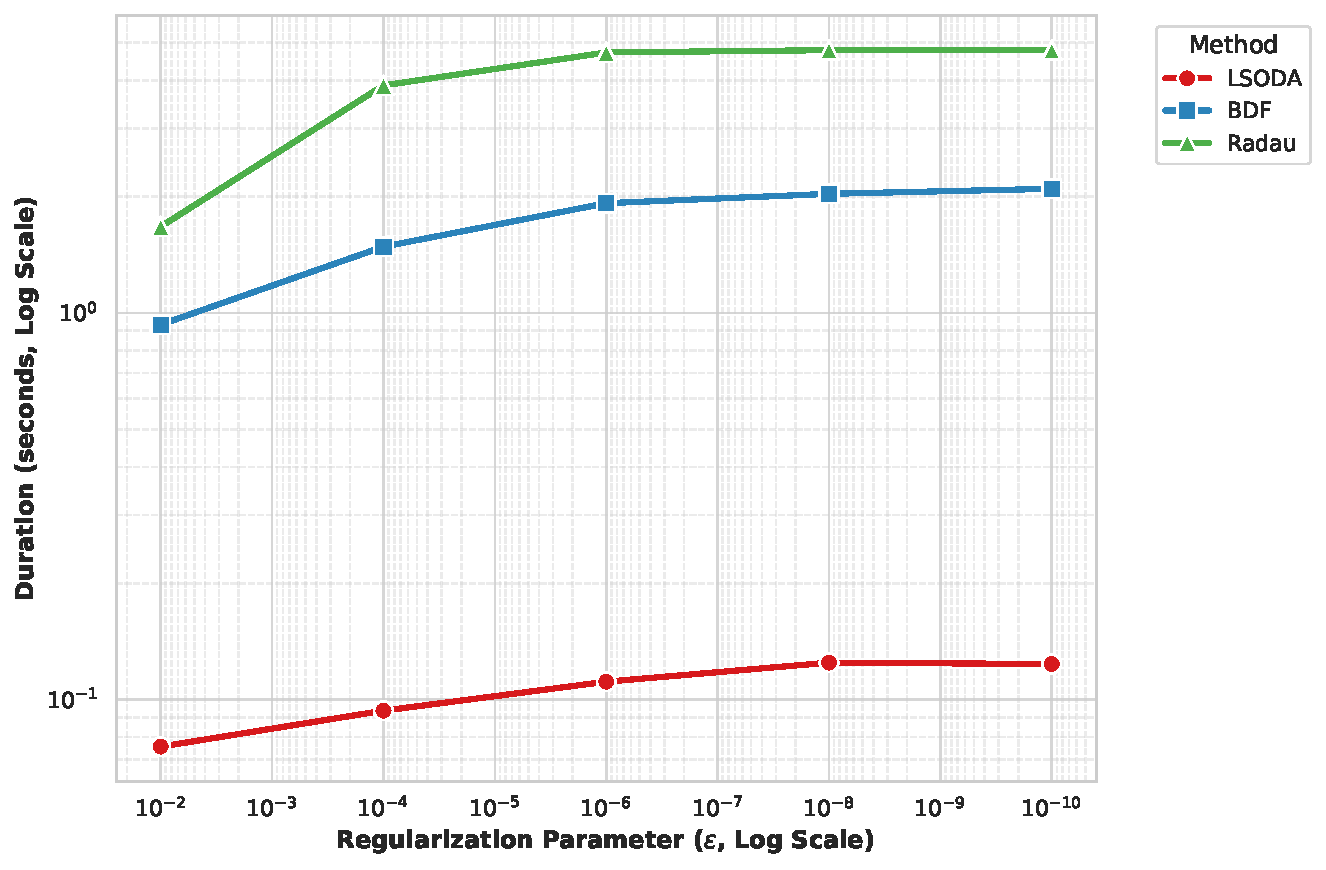
\includegraphics[width=\textwidth]{images/epsilon_sweep.pdf}
  \caption{Execution time scaling of LSODA, BDF, and Radau solvers against the regularization parameter \(\varepsilon\).}
  \label{fig:epsilon-sweep}
\end{figure}
